\documentclass[titlepage,a4paper]{article}

\usepackage{a4wide}
\usepackage[colorlinks=true,linkcolor=black,urlcolor=blue,bookmarksopen=true]{hyperref}
\usepackage{bookmark}
\usepackage{fancyhdr}
\usepackage[spanish]{babel}
\usepackage[utf8]{inputenc}
\usepackage[T1]{fontenc}
\usepackage{graphicx}
\usepackage{float}
\usepackage{listings}
\usepackage[table,xcdraw]{xcolor}
\usepackage{pdfpages}
\usepackage{tikz}
\usepackage{cprotect}
\usepackage{url}
\newcommand{\codigoMateria}{75.06/95.58}
\newcommand{\nombreMateria}{[75.06/95.58] Organización de datos}
\newcommand{\curso}{1}

\newcommand{\numeroTP}{1}
\newcommand{\tituloTP}{Trabajo práctico 2}
\newcommand{\descripcionTP}{Machine Learning}

\newcommand{\facultad}{Facultad de Ingeniería}
\newcommand{\universidad}{Universidad de Buenos Aires}
\newcommand{\cuatrimestre}{2do Cuatrimestre de 2020}


\pagestyle{fancy} % Encabezado y pie de página
\fancyhf{}
\fancyhead[L]{TP1 - Análisis Exploratorio}
\fancyhead[R]{[75.06/95.58]Organización de datos - FIUBA}
\renewcommand{\headrulewidth}{0.4pt}
\fancyfoot[C]{\thepage}
\renewcommand{\footrulewidth}{0.4pt}

\newcommand{\teammember}[3]{
	 #1 & #2 & \texttt{#3}\\
}

\begin{document}
\begin{titlepage} % Carátula
    \centering
      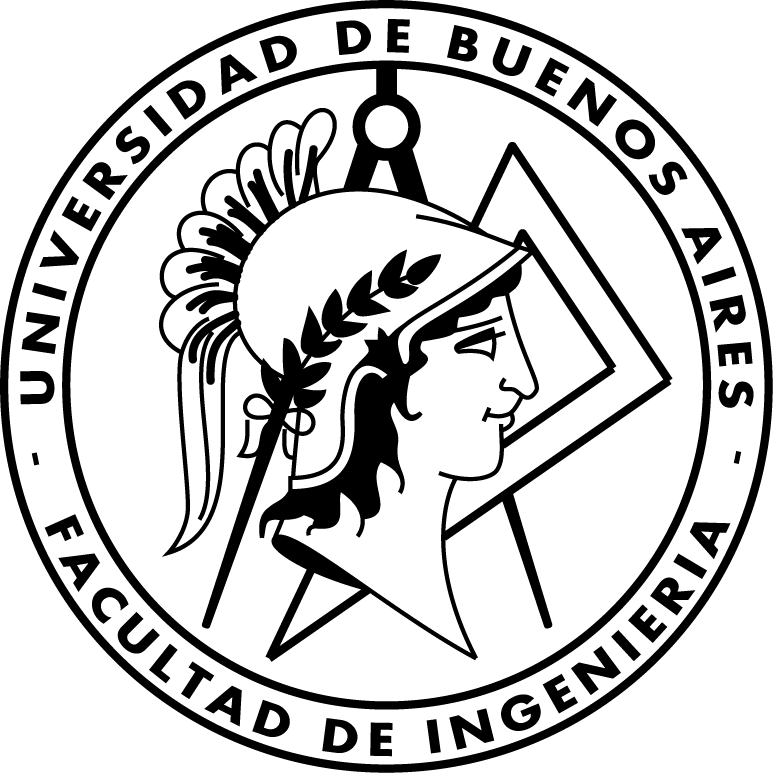
\includegraphics[scale = 0.75]{images/logo_fiuba.png}\\[1.0 cm]	% Logo universidad
      \textsc{\LARGE \universidad}\\[0.5 cm]	% Nombre universidad
      \textsc{\Large \facultad}\\[0.5 cm]	% Facultad
      \textsc{\large \cuatrimestre}\\[1.0 cm]	% Cuatrimestre
    \centering
    
     \textsc{\Large \nombreMateria}\\[0.5 cm] % Nombre materia
      \textsc{\large Curso \curso}\\[0.4 cm]	% Curso
      
      \rule{\linewidth}{0.2 mm} \\[0.4 cm]
      { \huge \tituloTP}\\[0.5 cm]
      { \huge \bfseries}
      { \huge \bfseries \descripcionTP}\\
      \rule{\linewidth}{0.2 mm} \\[1 cm]
      
     \resizebox{12cm}{!}{
        \begin{tabular}{ l  l  l}
          Padrón & Alumno & Email \\
          \hline
          \teammember{102914}{More, Agustín}{amore@fi.uba.ar}
      	\end{tabular}
  	}
  	
\end{titlepage}


\tableofcontents % Índice general
\newpage
\section{Introducción}\label{sec:intro}
El trabajo práctico consiste en analizar los datos provistos por la cátedra sobre una empresa ficticia `Frío Frío'. En base al análisis que se hizo en el trabajo práctico 1 (Análisis exploratorio) \cite{tp_analisis_exploratorio} adicionando un enfoque más profundo en la extracción de \textit{features} junto con la evaluación de modelos de \textit{Machine Learning}, se espera poder estimar la probabilidad de éxito de cada oportunidades.

El código y el material complementario se encuentra en el repositorio de github: \url{https://github.com/moreover22/datos/tree/main/tp2}

\section{Análisis previo}\label{sec:analisis_prev}

\subsection{Limpieza de datos}\label{subsec:limpieza_datos}
Durante el desarrollo del trabajo práctico 1, se realizó un análisis sobre el set de datos con la finalidad de extraer \textit{insights} junto con visualizaciones, que permitieron entender mejor el set. Para el desarrollo de este trabajo práctico, se retoma sobre lo ya estudiado en el primer informe, y se profundiza sobre las características o \textit{features} que serán luego utilizadas en los modelos predictores. Un paso clave para este estudio, fue reducir la complejidad del dataset, es decir, descartar aquellas columnas que no aportaban conocimiento sobre las oportunidades. Se obtuvieron varias columnas las cuales no variaban a lo largo de las oportunidades, es decir se mantenían constantes. En cambio, otras columnas, contenían datos redundantes o datos doblemente expresados a lo largo de distintas columnas.  Claramente, de este tipo de datos, no se puede obtener nueva información, con lo cual fueron descartadas. Estas columnas son: \verb|prod_category_a|, \verb|actual_delivery_date|, \verb|asp_currency|, \verb|asp|, \verb|last_activity|, \verb|submitted_for_approval| y \verb|asp_converted_currency|.


\subsection{Simplificación de categorías}\label{subsec:simp_cat}
Con el afán de seguir simplificando el dataset para poder tener una mayor facilidad al momento de manipular y entender el dataset, se analizan las columnas categóricas cuya cardinalidad es alta, pero con la particularidad de que la gran mayoría de los registros se encuentra encapsulada en una de las categorías, la simplicación consiste, entonces, en convertir una variable categórica en una categoría binaria. Ejemplos de esto son: \verb|category_b| (cuya clase principal abarca el $\%93.96$), \verb|brand| ($\%93.88$ clase mayoritaria), \verb|size| ($\%94.19$ pertenecen a la misma categoría).


\subsection{Target leakage}\label{subsec:targ_leak}
Al analizar las distintas características de cada oportunidad, al analizar en particular el campo \verb|sales_contract_no|, se puede ver que revela casi inmediatamente el \verb|stage| de la oportunidad, tal como lo muestra la figura \ref{fig:target_leakage}. Es muy importante que para las predicciones de los modelos de \textit{Machine Learning} no se tenga en cuenta esta característica, ni directamente (usando este campo como feature), ni indirectamente (usando este campo para encoding de otra variable). Si se llegara a utilizar, se obtendrían modelos con score sobre optimistas que luego en producción no responda de la manera esperada, ya que en un escenario real, al obtener una nueva oportunidad no se contara con esta información haciendo que los modelos fallen.

\begin{figure}[H]
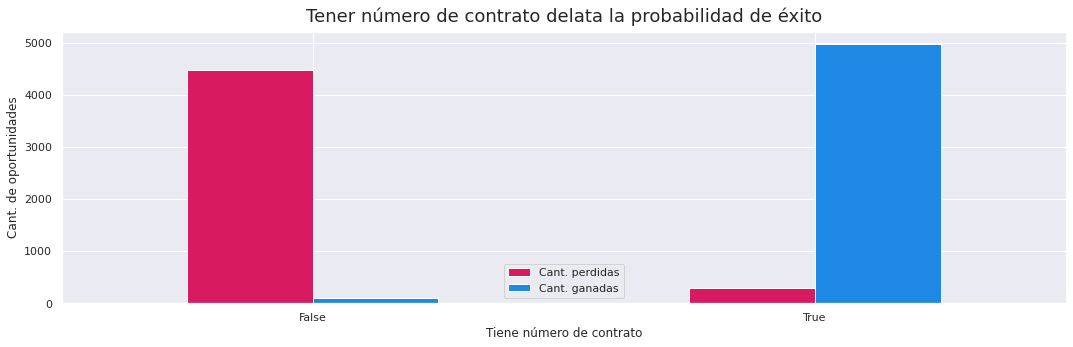
\includegraphics[width=0.8\textwidth]{images/targ_leak.png}
\cprotect\caption{\label{fig:target_leakage} Target leakage desde el atributo \verb|sales_contract_no|}
\end{figure}

Si bien no es correcto utilizar este feature para el entrenamiento del modelo, durante el trabajo, se lo utilizó para obtener una aproximación al feedback que brinda la competencia de kaggle, así pudiendo sobrepasar la limitación de cinco submits por día, además de poder obtener una respuesta mucho más rápida sin necesidad de persistirlo. Nuevamente, no se utilizó para ajustar los modelos, lo cual sería incorrecto, sino para sobrepasar las limitaciones de kaggle.


\section{Aplanado de dataset}\label{sec:aplanado_dataset}
Una vez pasada la primera iteración de manipulación del dataset, surge la necesidad de decidir cómo se realizará la predicción para cada oportunidad. El impedimento principal es que por cada oportunidad, se cuentan con varios registros en el dataset, esto hace que no haya una translación directa a los modelos predictivos. Se analizan dos acercamientos para superar esta complicación:

\subsection{Join-fit}\label{sub:joinfit}
La primera consiste en reducir del dataset a un registro por oportunidad, permitiendo así pasarlo directo a los modeles e inmediatamente poder utilizar los resultados. Para poder implementarlo, como primer paso se toman todas las características que son propias de la oportunidad, es decir que para todos los registros relacionados con una oportunidad, ese dato se mantiene constante. Luego de analizarlo, se determina que estos campos son: 

\begin{itemize}
    \item \verb|opportunity_id|,
    \item \verb|opportunity_name|,
    \item \verb|source|,
    \item \verb|opportunity_owner|,
    \item \verb|opportunity_created_date|,
    \item \verb|opportunity_type|,
    \item \verb|last_modified_date|,
    \item \verb|last_modified_by|,
    \item \verb|bureaucratic_code|,
    \item \verb|bureaucratic_code_0_approved|,
    \item \verb|bureaucratic_code_0_approval|,
    \item \verb|pricing_delivery_terms_approved|,
    \item \verb|pricing_delivery_terms_quote_appr|,
    \item \verb|account_name|,
    \item \verb|account_owner|,
    \item \verb|account_type|,
    \item \verb|account_created_date|,
    \item \verb|quote_type|,
    \item \verb|quote_expiry_date|,
    \item \verb|delivery_terms|,
    \item \verb|region|,
    \item \verb|territory|,
    \item \verb|billing_country|,
    \item \verb|total_taxable_amount|,
    \item \verb|total_taxable_amount_currency|,
    \item \verb|stage| 
\end{itemize}

Con estos campos, se crea un dataframe de oportunidades (que será utilizado en los modelos), donde existe una relación uno a uno entre registro y oportunidades. Por otra parte queda definido un dataframe de ventas donde se detallan los productos y sus características de cada uno. Una consecuencia inmediata es que los datos propios del producto no se estarían utilizando si solo se usa el dataframe de oportunidades en los modelos, con lo cual se agregan estadísticos de los productos que serán utilizados para las predicciones. Estos se detallarán con mayor detalle en la sección de Feature Engineering en las sección \ref{sec:feature_engineering}.

Cabe destacar que proceder con este método tiene como desventaja que la cardinalidad del dataset se reduce, es decir, la cantidad de muestras que utilizarán los modelos se ven reducidas. Otro inconveniente es que al solo considerar estadísticos del dataframe de ventas, se podría estar sobre simplificando y sobre estimando características que pueden llegar a ser importantes para la predicción.

Este proceso se resume en el diagrama de la figura \ref{fig:preproc_pipeline}.

\begin{figure}[H]
\centering
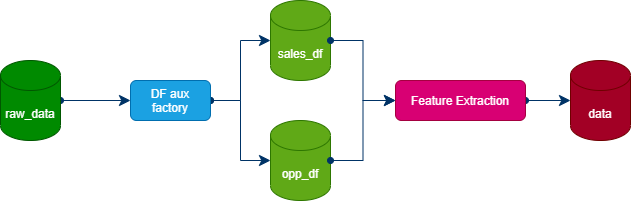
\includegraphics[width=0.9\textwidth]{images/preprocessing_pipeline.png}
\cprotect\caption{\label{fig:preproc_pipeline} Diagrama de preproceso de datos.}
\end{figure}

\subsection{Fit-join}\label{sub:fitjoin}
Otra alternativa, consiste en utilizar el dataframe tal cual está en los modelos (previo encoding, feature engineering, etc.) para luego, una vez que se obtiene la predicción, agrupar por oportunidades y sacar un promedio o Major voting.


\section{Feature Engineering}\label{sec:feature_engineering}

\subsection{Feature Extraction}
Como se optó seguir por la primer alternativa, join-fit, esto determinó en gran parte el tipo de features que se fueron descubriendo, y además cómo tratarlo en el dataset para utilizar los modelos. Cuando se trata de un feature propio de la oportunidad, se deja tal cual está en el dataframe (salvo que requiera algún otro procesamiento), en cambio si se trata de una cualidad de los productos dentro de la oportunidad, es decir algún feature que se extraiga del dataframe de \verb|sales|, para que sea funcional dentro del dataframe principal, se deben calcular estadísticos que describan la esencia de cada uno. Entre los cuales, dado un feature, para algunos se calculó la suma, se los contó, se calculó el promedio y/o se calculó la desviación standard.

Finalmente los features resultaron:

\subsubsection{Columnas categóricas}
\begin{itemize}
    \item \verb|bureaucratic_code|: Es una cualidad propia de la oportunidad, se tomó tal cual estaba en el dataset.
    \item \verb|account_type|: Intrínseco al cliente relacionado con la oportunidad.
    \item \verb|delivery_terms|: Caracteriza el envío de la oportunidad.
    \item \verb|region|: Brinda información geográfica general de la oportunidad.
\end{itemize}


\subsubsection{Columnas numéricas}
\begin{itemize}
    \item \verb|bureaucratic_code_0_approved|, \verb|bureaucratic_code_0_approval|: Flags del estado de la oportunidad burocráticamente.
    \item \verb|pricing_delivery_terms_approved|, \verb|pricing_delivery_terms_quote_appr|: Flags relacionadas con el envío.
    \item \verb|quote_type_binding|: Flag que determina el tipo de contrato.
    \item \verb|total_taxable_amount|: Es el total que cuestan los productos de la oportunidad.
    \item \verb|trf_mean|: Promedio del trf de los productos de la oportunidad.
    \item \verb|trf_sum|: Suma del trf de los productos de la oportunidad.
    \item \verb|trf_count|: Cuanta la cantidad de productos que hay en la oportunidad.
    \item \verb|planned_delivery_interval_mean|: Es el promedio del tiempo estipulado del envío de los productos.
    \item \verb|asp_ratio_mean|: Promedio de la tasa de conversión del asp. Si bien se toma el promedio, la varianza del radio por oportunidad se mantiene bastante bajo, implicando que es relativamente constante (esto se analiza en el notebook).
    \item \verb|total_amount_mean|: Es el precio promedio de los productos de la oportunidad.
    \item \verb|total_amount_sum|: Es el total a pagar en la oportunidad. Este valor debería coincidir teóricamente, con \verb|total_taxable_amount|, sin embargo no coincide, lo que explica el siguiente feature.
    \item \verb|amount_taxable_difference|: Es la diferencia entre \verb|total_taxable_amount| y \verb|total_amount_sum|. Esto generó que haya correlación entre estás variables, tal como muestra el gráfico de la figura \ref{fig:heatmap_corr}, con lo cual luego de probarlo se terminó removiendo.
\end{itemize}

\begin{figure}[H]
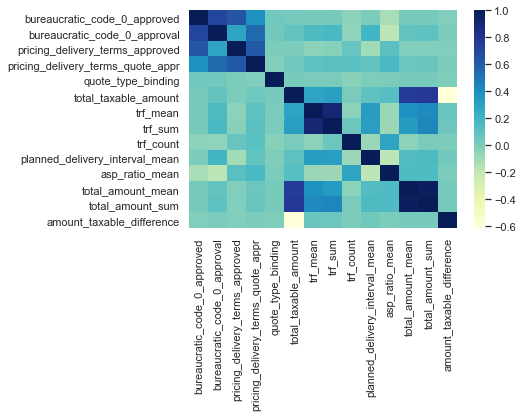
\includegraphics[width=0.8\textwidth]{images/correlation_numeric_values.png}
\cprotect\caption{\label{fig:heatmap_corr} Correlación entre las variables numéricas.}
\end{figure}

\subsection{Feature Selection}\label{sub:feature_selection}

Una vez definido los features y calculados y codificados, se entrena un modelo básico de árbol de decisión para poder determinar cuales son los features que más influyen positivamente en la predicción. Como primer paso, se entrena el modelo con el listado completo de features, adicionando una columna con valores random \cite{intr_machine_learning_with_python}. Una vez entrenado, se inspecciona el \verb|feature_importance| brindado por la librería de \textit{sklearn}, obteniendo los resultados de la figura \ref{fig:features_importance}.


\begin{figure}[H]
\centering
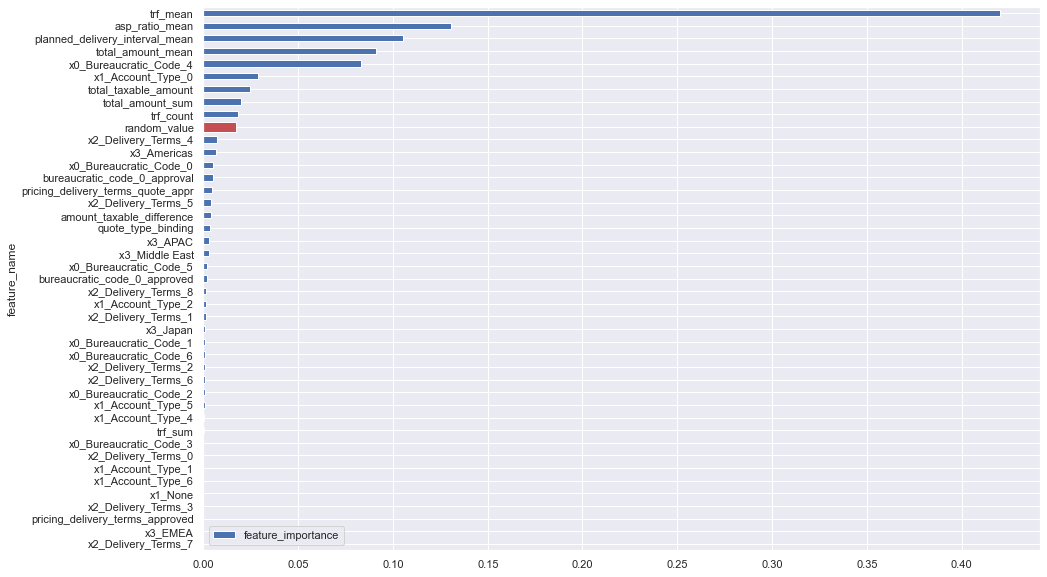
\includegraphics[width=0.9\textwidth]{images/feature_importance_dec_tree.png}
\cprotect\caption{\label{fig:features_importance} Feature importance con una variable random.}
\end{figure}

Las variables que se encuentran por debajo de la variable random, no están funcionando del todo bien para este modelo, ya que una variable que no tiene relación con las oportunidades tienen mayor prioridad al momento de predecir.

Para poder reducir la cantidad de columnas que no están ayudando en la predicción y pueden potencialmente introducir ruido o producir overfitting. Se parte de seleccionar las columnas que superan el umbral de la variable random, es decir, \verb|x1_Account_Type_0|, \verb|total_taxable_amount|, \verb|x0_Bureaucratic_Code_4|, \verb|total_amount_mean|, \verb|planned_delivery_interval_mean|, \verb|asp_ratio_mean| y \verb|trf_mean|. Luego para no descartar los demás features, se fueron agregando uno a uno los demás features y se conservaron aquellos que aumentan el \verb|score| y la métrica de \verb|log_loss|. Iterando sobre este \textit{algoritmo greedy}, se obtuvo finalmente, los features:

\begin{itemize}
    \item \verb|asp_ratio_mean|
    \item \verb|bureaucratic_code_0_approved|
    \item \verb|planned_delivery_interval_mean|
    \item \verb|pricing_delivery_terms_approved|
    \item \verb|total_amount_mean|
    \item \verb|total_taxable_amount|
    \item \verb|trf_mean|
    \item \verb|x0_Bureaucratic_Code_0|
    \item \verb|x0_Bureaucratic_Code_1|
    \item \verb|x0_Bureaucratic_Code_2|
    \item \verb|x0_Bureaucratic_Code_4|
    \item \verb|x0_Bureaucratic_Code_6|
    \item \verb|x1_Account_Type_0|
    \item \verb|x1_Account_Type_1|
    \item \verb|x1_Account_Type_4|
    \item \verb|x2_Delivery_Terms_2|
    \item \verb|x2_Delivery_Terms_3|
    \item \verb|x2_Delivery_Terms_4|
    \item \verb|x2_Delivery_Terms_6|
\end{itemize}

Una de las ventajas principales de reducir la cantidad de features es reducir el tiempo de entrenamiento y prevenir overfitting sobre features muy partículares que no permiten generalizar correctamente. Además, al reducir la cantidad de features, se requieren menos muestras en el dataset para poder entrenar coherentemente los modelos. Como desventaja, el razonamiento parte de algo que no necesariamente es cierto, ya que se toman los features importance del modelo de árbol de decisión que no necesariamente va a ser lo mismo para los demás modelos, pudiendo así perder features importantes para otro modelo. En particular, la mayoría de los modelos utilizados fueron basados en árboles, esperando así un comportamiento comparable entre los modelos. 

\section{Modelos de Machine Learning}\label{sec:modelos_machine_learning}
Una vez procesado el dataset y habiendo guardada las transformaciones necesarias para las predicciones sobre nuevas oportunidades, se evalúan distintos modelos para realizar las predicciones. La mayoría de los modelos son basados en árboles dada la naturalidad del problema, aunque este punto se retomará al final.

\subsection{Decision Tree}\label{sub:des_tree}
Este fue el primer modelo (fuera de los triviales) que se usó. Se obtuvo una gran diferencia entre este modelo y el anterior (modelo \textit{dummy} que asigna la probabilidad 1 para todas las oportunidades) pasando del score (score de kaggle) $16.98306$ a $2.51927$ luego de un tuneo básico de los parámetros. Este modelo cuenta con una gran ventaja frente los demás modelos de Machine Learning, este modelo es relativamente fácil de visualizar, tal como lo muestra la figura \ref{fig:plot_tree}. Cabe destacar que con este dataset es un modelo que se entrena bastante rápido, permitiendo hacer Grid Search para la búsqueda de hiperparámetros en un tiempo razonable. Esto es clave, ya que si no se regulan, es un modelo que tiende a overfitear, evitando que se pueda generalizar las predicciones. Los hiperparámetros que se pueden regular principalmente son \verb|max_depth| (profundidad máxima del árbol) y \verb|min_samples_split| (cantidad mínima de muestras para poder dividir un nodo). Ambos contribuyen a evitar el overfiting.

A pesar de todas las ventajas provistas, no fue el modelo con los mejores resultados, siendo así el mejor resultado obtenido con este modelo $0.67783$.

\begin{figure}[H]
\centering
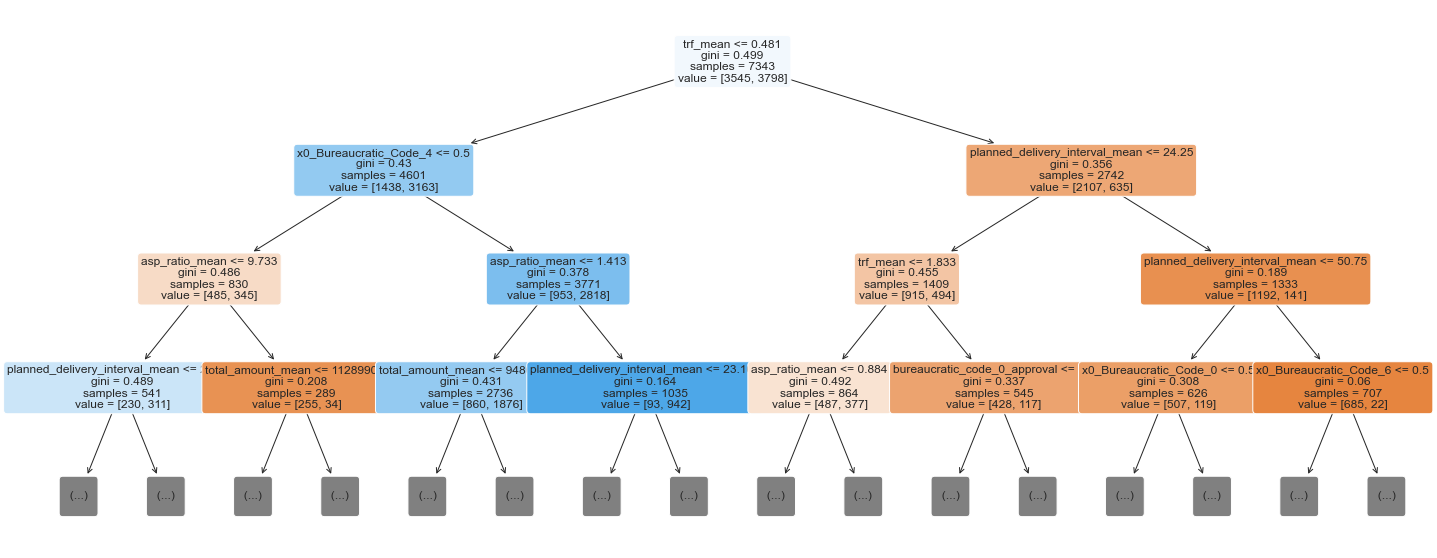
\includegraphics[width=1.1\textwidth]{images/des_tree_plot.png}
\cprotect\caption{\label{fig:plot_tree} Plot del DecisionTree}
\end{figure}


\subsection{CatBoost}\label{sub:cat_boost}
Este es el primer modelo que no pertenece a la librería \textit{sklearn} que se usa. A pesar de pertenecer a otra librería, la interfaz de los modelos siguen siendo igual que los demás modelos. Una de las cosas para mencionar es que admite entrenar el modelo sin tener que procesar las variables categóricas uno mismo, sino que el modelo automáticamente la codifica. Este modelo pertenece a la familia de gradient boosting, una de gran diferencia con los árboles de decisión anteriormente mencionada, es que utilizan \textit{weak learners}, es decir, árboles de baja profundidad, un nivel, pero en lugar de generar un árbol de generan \verb|n| estimadores, donde cada uno analizará alguna característica en particular. Se obtuvo un mejor resultado que en un árbol de decisión, pero el tiempo de entrenamiento fue significativamente superior, el puntaje comparado con otros modelos, fue de menor calidad.


\subsection{AdaBoost}\label{sub:cat_boost}
AdaBoost o Adaptative Boosting, es un modelo basado en árboles basado en boosting, tal como CatBoost, salvo que al ser Adaptative, al momento de armar los árboles, tiene en cuenta los desaciertos del árbol creado en el paso anterior. Dentro de los modelos de ensembles de árboles, este fue el que peor performance tuvo. Los hiperparámetros regulables son el \verb|learning_rate| y \verb|n_estimators|, es decir la cantidad de \textit{weak learners} usará internamente.

\subsection{lightGBM y XGBoost}\label{sub:lightgbm_xgboost}
Ambos algoritmos basados en árboles aplicando gradient boosting. Los resultados entre ambos fueron similares, aunque lighGBM fue más rápido de entrenar. Como ambos modelos cuantan con una gran cantidad de hiper-parámetros para descubrir, se fueron optimizando localmente uno por uno, dejando fijo a los demás, si bien no es necesariamente el resultado más óptimo, pero es practicable en un tiempo razonable. Ambos difieren en la forma en que arman los árboles, XGBoost arma los árboles por niveles, mientras que lighGBM se focaliza sobre las hojas \cite{lightgbm_vs_xgboost}. En combinación ambos quedaron en segundo lugar de mejores resultados.

\subsection{Random Forest}\label{sub:randomforest}

Un Random Forest consiste en un ensemble de Decision Tree, donde cada árbol es independiente de los demás. Contar con varios árboles previene que se genere overfitting, si es controlada correctamente la profundidad de los mismos. Este modelo terminó siendo el que mejor resultados brindó (dentro de los modelos individuales). Similar a los modelos anteriores, al contar con una gran cantidad de hiper-parámetros para tunear, terminó siendo impracticable realizar Grid search sobre todos los posibles parámetros, teniendo así que regular localmente las variables. 

\begin{figure}[H]
\centering
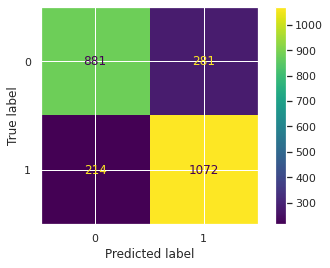
\includegraphics[width=0.6\textwidth]{images/conf_mat_rand_for.png}
\cprotect\caption{\label{fig:plot_tree} Confusion matrix del modelo Random Forest}
\end{figure}

\subsection{Ensembles}\label{sub:ensembles}
Una vez probado y entrenado distintos modelos se propone combinarlos generando así un nuevo estimador, que combine los descubrimientos de cada modelo.

\subsubsection{VotingClassifier}\label{subsub:voting}
Este ensemble consiste en realizar una predicción con cada uno de los estimadores que componen a el clasificador y luego promediarlo. En particular se utilizan los tres modelos que mejores resultados han dado individualmente: \verb|Random Forest|, \verb|XGBoost| y \verb|lightGBM|. Este ensemble no cuenta con parámetros para tunear, salvo el parámetro \verb|voting|, que como lo que se quiere hacer es predecir una probabilidad, se debe usar \verb|voting='soft'|.

\begin{figure}[H]
\centering
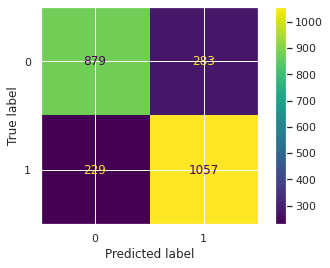
\includegraphics[width=0.4\textwidth]{images/conf_mat_voting_ens.png}
\cprotect\caption{\label{fig:plot_tree} Confusion matrix del modelo VotingEnsemble con los clasificadores \verb|Random Forest|, \verb|XGBoost| y \verb|lightGBM|}
\end{figure}

\subsubsection{BaggingClassifier}\label{subsub:bagging}
Como última capa del pipeline, se agrega un Bagging ensemble que tomará como estimador base el VotingClassifier de la sección \ref{subsub:voting}, este ensemble entrenará este modelo (y a su vez a los modelos internos de VotingClassifier), con subconjuntos del dataset original, generan así \verb|n| estimadores donde luego se promediarán las predicciones. Este ensemble es útil para reducir la varianza del modelo anterior \cite{bagging_ensembre}, introduciendo una componente aleatoria, particularmente importante al armar los árboles de boosting.


\begin{figure}[H]
\centering
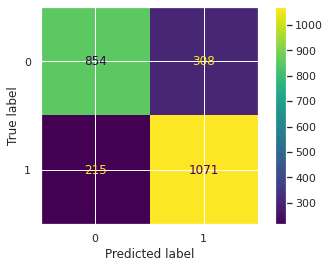
\includegraphics[width=0.4\textwidth]{images/conf_mat_bag_ens.png}
\cprotect\caption{\label{fig:plot_tree} Confusion matrix del modelo VotingEnsemble con los clasificadores \verb|Random Forest|, \verb|XGBoost| y \verb|lightGBM|}
\end{figure}

Aunque las matrices de confusión parecerían estar incrementando las clasificaciones erróneas, el \verb|log_loss|, fue decreciendo con los ensenbles, se puede explicar que los modelos en los ensembles tienen mayor seguridad en sus predicciones.

El esquema de la figura \ref{fi:model_pipeline} resume la estructura del modelo completo.
\begin{figure}[H]
\centering
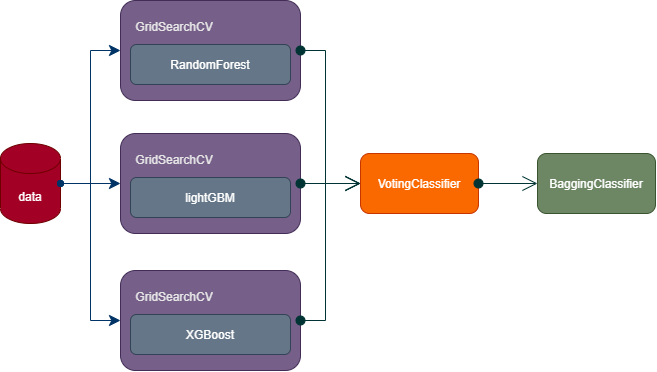
\includegraphics[width=0.9\textwidth]{images/model_pipeline.png}
\cprotect\caption{\label{fig:model_pipeline} Modelo de predicción}
\end{figure}


\section{Conclusiones}\label{sec:conclusiones}
Tal como se pronostica constantemente, gran parte del proceso de Machine Leraning se concentra en la manipulación de datos y feature engineering, ya que el proceso de entrenamiento y de corroboración es el mismo a lo largo de los distintos modelos, inclusive si se tratan de librerías independientes. Es cierto que hay modelos cuya etapa de entrenamiento puede tomar un largo periodo de tiempo, cosa que se discutirá en las oportunidades de mejora. 

Muchas veces, lo que uno cree que puede llegar a funcionar, hace que la performance de los modelos de disminuya, haciendo que muchas veces hasta que no se prueba un feature no se tiene completa certeza de si va a funcionar correctamente. Además, si no se es metódico en las cosas que uno prueba puede terminar perdiendo avances previos que no podrá recuperar o bien terminar en un ciclo de cosas que ya se probaron con anterioridad.

\subsection{Oportunidades de mejora}\label{sub:opp_mejoras}
Llegando al final de la realización del trabajo, se descubren distintas decisiones que se podrían haber tomada en una etapa más temprana que podrían haber llevado a la elaboración de un sistema de predicción mucho más robusto. Un punto pendiente es siempre el agregado y optimización de features, ya que muchos modelos terminan dando puntajes muy parecidos y solo mejoran cuando se manipulan los features de una forma más óptima.

Todos los modelos fueron basados en árboles, dentro de su gran familia de variantes, algo que podría hacer un predictor más interesante es combinar distintas familias de modelos, ya que le agregan más dinamismos y pueden encontrarse patrones que no son descubiertos por los modelos de árboles.

Una propuesta interesante es utilizar los acercamientos de \verb|join-fit| (sección \ref{sub:joinfit}) y \verb|fit-join| (sección \ref{sub:fitjoin}) para luego combinar los resultados, generando así modelos que fueron formados completamente distintos sobre el mismo dataset, consiguiendo así descubrir distintos patrones que uno no los logró detectar, pero el otro quizás sí.

Otra optimización importante que hubiera hecho el proceso de investigación mucho más eficiente, es separar el análisis en distintos notebooks, permitiendo tanto así la reutilización, como paralelizar tareas fácilmente y poder seguir trabajando sobre otros aspectos del trabajo. Una posible propuesta es la siguiente: 
\begin{itemize}
    \item Limpieza de datos
    \item Creación de dataframes auxiliares
    \item Features extraction
    \item Features selection
    \item Model training
    \item Búsqueda de hiper-parámetros
\end{itemize}

\newpage
\appendix
\section{Ejecución del \textit{script} de los modelos}

Se puede descargar el código desde el \href{https://github.com/moreover22/datos/tree/main/tp2}{repositorio de Github}.

Para poder correr el \textit{script} que genera el análisis y los gráficos, primero hay que instalar las librerías necesarias, se puede hacer mediante la herramienta \verb|pip| \footnote{Herramienta \textbf{pip}: \url{https://pypi.org/project/pip/}} con el siguiente comando:

\begin{verbatim}
    pip install -r requirements.txt
\end{verbatim}

Para realizar realizar una instalación más ordenada y sin tener conflicto de versiones es recomendable usar un entorno virtual \footnote{Entorno virtual de python (venv): \url{https://docs.python.org/3/library/venv.html}}
Una vez finalizada la instalación, para ejecutar el programa:

\begin{verbatim}
    python tp_datos_2c2020.py
\end{verbatim}


Si se quiere evitar la parte de instalación se puede ejecutar el \href{https://colab.research.google.com/drive/1cIS9cFXRtDXCx1CANUsSSSPxUlPxwVtn?usp=sharing}{notebook} desde la herramienta \textit{Google Colab} \footnote{Google Colab \url{https://colab.research.google.com/}}.

\newpage
\begin{thebibliography}{9}



\bibitem{tp_analisis_exploratorio}
\cprotect\textit{Trabajo práctico 1 | Análisis exploratorio}. 
\url{https://github.com/moreover22/datos/tree/main/tp1}

\bibitem{intr_machine_learning_with_python}
\cprotect\textit{Introduction To Machine Learning With Python - Sarah Guido}.

\bibitem{lightgbm_vs_xgboost}
\cprotect\textit{XGBoost vs LightGBM - Sefik Ilkin Serengil}. 
\url{https://sefiks.com/2020/05/13/xgboost-vs-lightgbm/}


\bibitem{bagging_ensembre}
\cprotect\textit{BaggingClassifier - scikit-learn}. 
\url{https://scikit-learn.org/stable/modules/generated/sklearn.ensemble.BaggingClassifier.html#sklearn.ensemble.BaggingClassifier}

\end{thebibliography}


\end{document}